%%%  Bryan P Dannowitz
%%%  University of Illinois
%%%  10/19/11

\documentclass[11pt]{article}

\setlength{\topmargin}{-0.375in}
\setlength{\oddsidemargin}{-0.125in}
\setlength{\evensidemargin}{-0.125in}
\setlength{\textwidth}{6.5in}
\setlength{\textheight}{8.75in}

\usepackage{subfigure}
\usepackage{graphics}
\usepackage{wrapfig}
\usepackage{amsmath}
\usepackage{amsfonts}
\usepackage{amssymb}
\usepackage{ifpdf}

\newif\ifpdf
\ifx\pdfoutput\undefined
        \pdffalse
\else
        \pdfoutput=1
        \pdftrue
\fi

\ifpdf
        \usepackage[pdftex,
                colorlinks=true,
                urlcolor=blue,
                linkcolor=blue,
                citecolor=blue,
                ]{hyperref}
        \hypersetup{
                pdftitle={A Drell-Yan study of Short Range Correlations and the Nuclear EMC Effect at SeaQuest}
                pdfauthor={Bryan Dannowitz}
                pdfsubject={Nucleon Structure}
                pdfkeywords={EMC, Drell-Yan, Structure Functions}
                }
        \usepackage[pdftex]{graphicx}
\else
%        \usepackage[dvips]{hyperref}
\usepackage[dvips]{graphicx}

\usepackage[dvips]{graphicx,color}
\usepackage[dvipdfm]{hyperref}
\hypersetup{%
pdftitle={A Drell-Yan Study of the Nuclear EMC Effect at SeaQuest},
pdfauthor={B. Dannowitz},
pdfsubject={Nucleon Structure in a Nucleus},
pdfkeywords={QCD, Partons, EMC Effect, SRC, Drell-Yan},
colorlinks,linkcolor={blue},citecolor={blue},urlcolor={blue},
}%
\fi

\title{{\Large \textbf A Drell-Yan study of Short Range Correlations and the Nuclear EMC Effect at SeaQuest}}%
\author{B. Dannowitz\\%
  Advisor: Naomi Makins\\%
  University of Illinois At Urbana-Champaign\\%
  \href{mailto:dannowi1@illinois.edu}{\emph{dannowi1@illinois.edu}}}

\date{\normalsize{October 19th, 2011}}

\begin{document}
  \maketitle
  \begin{abstract}
The European Muon Collaboration found that the distribution of quarks in a nucleon differs significantly from the distribution of quarks in a nucleus. This phenomenon has been studied in depth over the years via Deep Inelastic Scattering (DIS), but the current amount of Drell-Yan data on this subject is very limited. Promising theoretical and experimental progress has also been made providing evidence that the EMC effect is attributable to high-momentum nucleons, most of which can be accounted for by considering nucleon-nucleon Short Range Correlations (SRC's).  Previous experiments (E772) extend only from $0.04<x_2<0.3$ with the "EMC effect" region only \emph{beginning} at $x_2\approx0.3$. The SeaQuest experiment at Fermilab is well-poised, with its high luminosity and relatively low beam energy, to introduce a large volume of statistics for a considerably large $x_2$ range ($0.1<x_2<0.45$).
  \end{abstract}

\thispagestyle{empty} 

\newpage

\tableofcontents

\newpage

\begin{figure*}
    \centerline{
    \mbox{\includegraphics[width=4.50in]{DIS-DY.png}}
    }
    \caption{(A) Deep inelastic scattering (DIS) is a $t$-channel interaction which uses the emission of a virtual photon to probe the target hadron. (B) The similar Drell-Yan (DY) process, using the $s$ channel version of the DIS interaction, via annihilation of a beam quark with an anti-quark from the target hadron.}
    \label{fig:dis-dy}
\end{figure*}

\section{Introduction: Drell-Yan and the Distribution of Quarks}

Nucleon structure is still today one of the great frontiers of nuclear physics.  The primary tool used to probe the parton distribution has been Deep Inelastic Scattering (DIS), which is the scattering of a charged lepton off of a nucleus by the exchange of a virtual photon.  As the energy of the exchanged photon increases, the scattering becomes inelastic and is able to resolve the partonic substructure of hadrons.  As useful as this has been, DIS is only sensitive to momentum and charge of the partonic structure.

In 1970, S. Drell and T.M. Yan were the first to study the process in which high-mass lepton production occurs as a result of inelastic hadron-hadron collisions \cite{Drell:1970wh}.  This so-called "Drell-Yan" (DY) process is identified to be the result of a quark-antiquark annihilation into a virtual photon which then decays into a lepton pair. 

This process, as you see in Figure \ref{fig:dis-dy}, is the \emph{s}-channel counterpart to DIS's \emph{t}-channel process.  Similarly Drell-Yan can give a complementary view of the nucleon's parton distribution. The differential cross section that we will be using is in terms of the fractional momentum variables, $x_1$ and $x_2$, which represent the fraction of the respective hadron's momentum carried by the beam quark and target anti-quark, respectively.

To begin, we start with the annihilation cross section for $e^+e^- \rightarrow \mu^+\mu^-$ and simply add a color factor of $\frac{1}{3}$ since only like flavor-antiflavor quarks will annihilate, and use the charge $e_i^2$ for quark flavor $i$ \cite{duan-2007-50}. Other variables referred to in Eq \ref{eq:DY-cross1} and \ref{eq:DY-cross2} and more are defined in Table \ref{tab:var}.

\begin{equation}
	\frac{d\hat{\sigma}}{dM} = \frac{8 \pi \alpha^2}{9M}e_i^2\delta(\hat{s} - M^2)
	\label{eq:DY-cross1}
\end{equation}

The hadronic Drell-Yan differential cross section can be obtained from this by the convolution of the above cross section with the quark distributions in the beam and target.

\begin{equation}
	\frac{d^2\sigma^{DY}}{dx_1x_2}=\frac{8\pi\alpha^2}{9sx_1x_2 K(x_1,x_2)}
	 \sum_{i}e_i^2[q_i^b(x_1)\bar{q}_i^t(x_2)+
	\bar{q}_i^b(x_1)q_i^t(x_2)]
\label{eq:DY-cross2}
\end{equation}

 \begin{table}[h]
  \begin{tabular}{ccl}
  Variable&Description\\ \hline \hline
  $\alpha$ & The fine structure constant \\
  $K(x_1,x_2)$ & High-order QCD correction term \\ \hline
  $\sqrt{s}$ & The center of mass energy of the hadronic collision \\
  $\sqrt{\hat{s}}$ & The center of mass energy of the $q\bar{q}$ collision \\
  $Q^{2}$ & The four-momentum of the intermediate time-like photon, squared \\ 
  $q_i^{t/b}(x)$ & The quark number density in the nucleon of the target/beam \\ \hline \hline
  \end{tabular}
  \caption{Kinematic variables relevant to the Drell-Yan process .}
  \label{tab:var}
  \end{table}


In addition to the leading-order DY term, there are high-order QCD corrections to consider. These have been studied and accounted for up to $O(\alpha_s)$ and $O(\alpha_s^2)$. These include contributions from high-order $q\bar{q}$ annihilation $(q \bar{q} \rightarrow \gamma * + g)$ and gluon Compton scattering $(q + g \rightarrow \gamma * + q)$ as seen in Figure \ref{fig:nlo-dy} \cite{duan-2007-50}. The cumulative effect is denoted in the cross section as the $K(x_1,x_2)$ factor, which can vary between 1.6 and 2.8.  For our $x_1$ and $x_2$ range, $K \sim 1.6$.

\begin{figure*}[h]
    \centerline{
    \mbox{\includegraphics[width=5.00in]{DY.jpeg}}
    }
    \caption{The Drell-Yan process has a large range of higher-order QCD corrections that need to be accounted for. (A) and (B) are high order $q\bar{q}$ annihilations, and (C) and (D) are gluon "Compton scattering" terms.}
    \label{fig:nlo-dy}
\end{figure*}

Now the question is: what can the Drell-Yan process tell us that the well-exercised DIS scattering cannot? The core answer to that is that DIS is not intrinsically sensitive to flavor, whereas DY is. However, to answer the question fully, we must discuss the distribution of quarks in a nucleon.  

Let's say that we have two hadrons A and B colliding; a parton of type \emph{a} ($u, d, s, g$, etc.) comes from A and carries with it a fraction of A's momentum ($x_A$).  The same goes for hadron B; a parton of type \emph{b} comes from B and carries momentum fraction $x_B$. Now, the probability of finding the discussed parton from A is given by $f_{a/A}(x_A)dx_A$. Likewise, the probability of finding the discussed parton from B is $f_{b/B}(x_B)dx_B$.  

These \emph{structure functions}, $f_{a/A}(x)$ are called the \emph{parton distribution functions} (PDF's), and they have been the focus of a great deal of experiments over the years by several collaborations. Due to the complex nature of lattice QCD, these PDF's are determined empirically, with only a few rules based in theory. It is important to note that there is normally a $Q^2$ dependence of these PDF's. At high enough $Q^2$, as it is in the case of our experiment, the PDF's no longer scale with $Q^2$ \cite{Seely:2009gt}.  That is, for a given \emph{x}, the PDF is independent of $Q^2$.

An important metric to observe is the probability that a parton \emph{a} carries a momentum fraction $x_A$ in its hadron $A$.  This can be represented by the following expression: $x_A f_{a/A}(x_A)dx_A$. For Drell-Yan interactions in the study proposed here, we are interested in the momentum distribution amongst the quarks in the proton.  The CTEQ collaboration has collected data from many experiments, yielding the model represented in Figure \ref{fig:pdf} \cite{Pumplin:2002vw}.

\begin{figure}
\centering
\mbox{
	\subfigure[The parton distribution function describing the momentum carried by different types of quark in the proton.]{
\includegraphics[width=0.40\linewidth]{parton-dist.jpg}
\label{fig:pdf}	}\quad
	\subfigure[The ratio of cross sections (per nucleon) as a function of the target's fractional momentum, $x_2$.  The EMC Effect region, $0.3<x_2<0.6$ is the phenomenon discussed here.]{
\includegraphics[width=0.53\linewidth]{EMC_EMC.jpeg}
\label{fig:emc} }
}
\caption{The proton's momentum distribution and the EMC Effect, with key regions highlighted.}
\label{fig:pdf_emc}
\end{figure}

Looking to Figure \ref{fig:pdf} we see that at $x>0.1$, $u$ and $d$ quarks dominate $\bar{u}$ and $\bar{d}$ quarks.  This is key, because this means that, for SeaQuest where we have high $x_1$ and lower $x_2$, the Drell-Yan process is probabilistically dominated by a quark from the beam annihilating with an antiquark from the target. All antiquarks that exist in the target nucleons must come from what are called the \emph{sea quarks}, or the virtual $q\bar{q}$ pairs that pop in and out of existence amongst the gluons and valence quarks. 

As we will discuss in the next section, partons in a bound nucleon behave differently than partons in a free nucleon. By studying Drell-Yan in nuclear targets, we can investigate the degree to which this modification is the result of a modification to the quark sea.

\section{Phenomenological Foundation}
\subsection{The EMC Effect}

The European Muon Collaboration, in 1983, measured the DIS cross section per nucleon ratios of $Fe$ to $D$ over a large kinematic range.  The result, as seen in the top right of Figure \ref{fig:emc} came as quite a surprise.  It was revealed that the structure function of a nucleon bound in a nucleus differs fundamentally from that of a free nucleon  \cite{Aubert:1983xm}.  This difference was not a simple or small effect either; the cross section per nucleon of a nucleus showed to be smaller than that of deuterium at very low $x_2$, greater than deuterium at $0.1<x_2<0.2$, and then steadily less than deuterium for $0.2<x_2<0.6$. 

This complex, unexplained behavior opened up a new field of research and theoretical work. Following suit, the different aspects of this nuclear modification garnered some common nicknames.  The region where $x_2<0.1$ became known as \emph{"Nuclear Shadowing"}, the transition region of $0.1<x_2<0.2$ is known as \emph{"Anti-shadowing"}, and the linear decline in the ratio of cross sections between $0.2<x_2<0.6$ is generally referred to as the \emph{"EMC Effect"} \cite{Geesaman:1995yd}.

The phenomenon was simple -- DIS off of a bound nucleon was not the same as off of a free nucleon -- but hundreds of theoretical papers were written attempting to explain it away, from multiquark ($6q$) clusters to the exchange of virtual pions in the nucleus. Some have joked that EMC should stand for \emph{"Every Model is Cool"}. The focus of recent work (and this paper) is on the "EMC Effect" region, characterized by the distinctly linear downward slope.

Recent experiments at Hall C at JLab and SLAC suggest the following regarding the EMC Effect \cite{Seely:2009gt}:
\begin{itemize}
\item
It is $Q^2$-independent
\item
It's x-dependent shape is universal (across various nuclei)
\item
The magnitude (slope) of the effect varies with A
\item
It thereby might be related to nuclear density
\end{itemize}

In parallel to this effort, many researchers were working on high-momentum nucleons and short range correlations (SRC's), neither aware yet of their common ground.

\subsection{Short Range Correlations}

\begin{wrapfigure}{r}{0.45\textwidth}
  \begin{center}
    \includegraphics[width=0.43\textwidth]{src.png}
  \end{center}
  \caption{Density of high-momentum nucleons \cite{PhysRevC.76.055206}}
  \label{fig:src}
\end{wrapfigure}

Between nucleons, there is a familiar potential that can be described by the usual short-range (1fm) repulsion along with an intermediate- to long-range attractive tensor force. When, by happenstance, two nucleons find themselves at a short distance from one-another, they become correlated via the short-range repulsive (coulomb) force. The immediate result is for them to accelerate away from each other rapidly, carrying with them a large amount of momentum. This phenomenon is called "NN-SRC", or Nucleon-Nucleon Short Range Correlations. These are the results of two (2N-SRC) or three (3N-SRC) or more nucleons getting too close together.

Ciofi, \emph{et al.} studied the density of high-momentum nucleons in heavy nuclei.  Due to the mean field of the nucleus, the momentum density was expected to drop off smoothly. What they found instead was a surprising divergence from the mean field at $P \sim 0.3 GeV/c$. In Figure \ref{fig:src}, you can see this manifested the "elbow" in the momentum density. Ciofi theorized that this high density in high momentum nucleons could be caused by NN-SRC, as described above \cite{PhysRevC.53.1689}.

Subsequent studies were performed via deep inelastic scattering, investigating the nature of these NN-SRC's. In 2003, Tang, \emph{et al.} at EVA / BNL performed a series of knock-out measurements on $^{12}C$, firing a proton at the nuclear material, measuring when two or more lone nucleons were knocked out, identified them, and measured their energy \cite{PhysRevLett.90.042301}.  The results stated that out of all the nucleons in $^{12}C$, approximately 20\% were in correlated pairs. Of those correlated pairs, $\sim90\%$ consisted of neurton-proton SRC pairs, while $\sim 5\%$ were in proton-proton and neutron-neutron SRC pairs. More importantly, though only 20\% of the nucleons are 2N-SRC correlated pairs, they carry \emph{80\%} of the nucleus' kinetic energy \cite{Subedi:2008zz}.

Naturally, if one is looking to study NN-SRC's, they might likely look to the density of nucleons in the nuclei.  Common sense dictates that the more dense the nuclei, the more likely for there to be more short-range interactions.  Seely, \emph{et al.} did just this and compared the scaled nuclear density to the EMC slope \cite{Seely:2009gt}. The results, as seen in Figure \ref{fig:density} are promising, but inconclusive, as $^9Be$ is far off of the possible trend that the light nuclei form.  However, due to the unique nuclear arrangement of $^9Be$, which is likely arranged similar to two alpha particles and a neutron, the average nuclear density does not well reflect the local densities that the nucleons experience.

Egiyan \emph{et al.} were also investigating two- and three-nucleon SRC probabilities at high Bjorken-x. Bjorken-x ($x_B$) is a scaling variable often used in DIS  (Figure \ref{fig:dis-dy}) and inclusive scattering, where 
\begin{equation}
	x_B = \frac{Q^2}{2m\omega}
\end{equation}

\begin{wrapfigure}{l}{0.45\textwidth}
  \begin{center}
    \includegraphics[width=0.43\textwidth]{density.png}
  \end{center}
  \caption{Scaled nuclear density vs. EMC Effect slope \cite{Seely:2009gt}}
  \label{fig:density}
\end{wrapfigure}

where $Q^2$ is the momentum transfer to the system, $\omega$ is the energy transfer, and m is the mass of the proton. Since m is always the mass of the proton, and a given parton in a large nuclei may have a large share of the total momentum at some point, it has an allowed range of $0\le x_b \le A$. We see in Figure \ref{fig:scale} that at high $x_B$ that the the EMC ratio plateaus at $x_B \sim 1.5$.  The ratios of the per nucleon inclusive cross sections for the two nuclei is the probability that one would find high-momentum nucleons in those two nuclei.  Seeing as how most of high-momentum nucleons are caused by NN-SRC's, the value at which each nuclei's ratio first plateaus is often referred to as the "SRC Scale Factor," and it is different for each nuclei.

\begin{figure}
\centering
\mbox{
	\subfigure[The "SRC Scale Factor", $a_{2}(A/d)$, is the first plateau in the ratio \cite{PhysRevLett.96.082501}]{
\includegraphics[width=0.52\linewidth]{src_scale.png}
\label{fig:scale}	}\quad
	\subfigure[The SRC Scale Factor vs. EMC Effect slope \cite{Weinstein:2010rt}]{
\includegraphics[width=0.42\linewidth]{correlation.png}
\label{fig:correlation} }
}
\caption{The SRC Scale Factor and its strong correlation to the EMC slope.}
\label{fig:src_emc}
\end{figure}

As we see this newly-declared SRC Scale Factor correlates very well with its own corresponding EMC slope (Figure \ref{fig:correlation}), it becomes clear that there must be some link between the two phenomenon.

\subsection{Connecting the Phenomenology: High-Momentum Nucleons}

When you look at how these SRC scale factors line up so precisely with the EMC ratio's slope, one can draw a general conclusion:
\begin{itemize}
\item
Higher SRC scale factors correspond to higher momentum nucleons in nuclei with larger local densities
\item
 The nuclei's EMC ratio slope scales linearly with the SRC scale factor
\item
The EMC effect is a modification of the nucleon structure when in a nucleus
\item
Therefore, it's likely that this modification is due to high-momentum nucleons.
\end{itemize}

In fact, Ciofi \emph{et al.} entertain this notion in their theoretical work on how nucleons with high \emph{virtuality} modify the nucleon wave function \cite{PhysRevC.76.055206}. Nucleon virtuality is a term used to express how much off-shell a particle is: $v = P^2 - m^2$ where P is the particle's four-momentum.

Ciofi shows that a more off-shell nucleon carries with it a modification of the radius of its form factor (charge distribution), making it more susceptible to deep inelastic processes and less to quasielastic processes. Also, Ciofi expresses that nucleons can be of two extremes: Blob-Like Configurations (BLC) which have an infinite number of configurations that all interact differently in the nuclear medium, and then there are Point-Like Configurations (PLC) which are rare configurations consisting of just three quarks nearby each other. It is then shown that in a nuclear medium, for a nucleon with large virtuality, the energy differences between BLC's and the rare PLC's are increased, thereby suppressing PLC's \cite{PhysRevC.76.055206}.

The interesting fact to note about this suppression of PLC's is that it would lead to a modification of the valence quarks, which may manifest itself very bluntly (i.e. no EMC effect slope) due to our reliance on the nuclear target's sea quarks.

\section{Measurements}

\begin{figure}
\centering
\mbox{
	\subfigure[Fermilab experiment E772 results; nuclear to deuterium cross sections per nucleon for $C, Ca, Fe, Sn, W$ \cite{Alde:1990im}]{
\includegraphics[width=0.4\textwidth]{e772.png}
\label{fig:e772}	}\quad
	\subfigure[The projected range and error of SeaQuest for the $Fe/D$ cross section against E772's results.]{
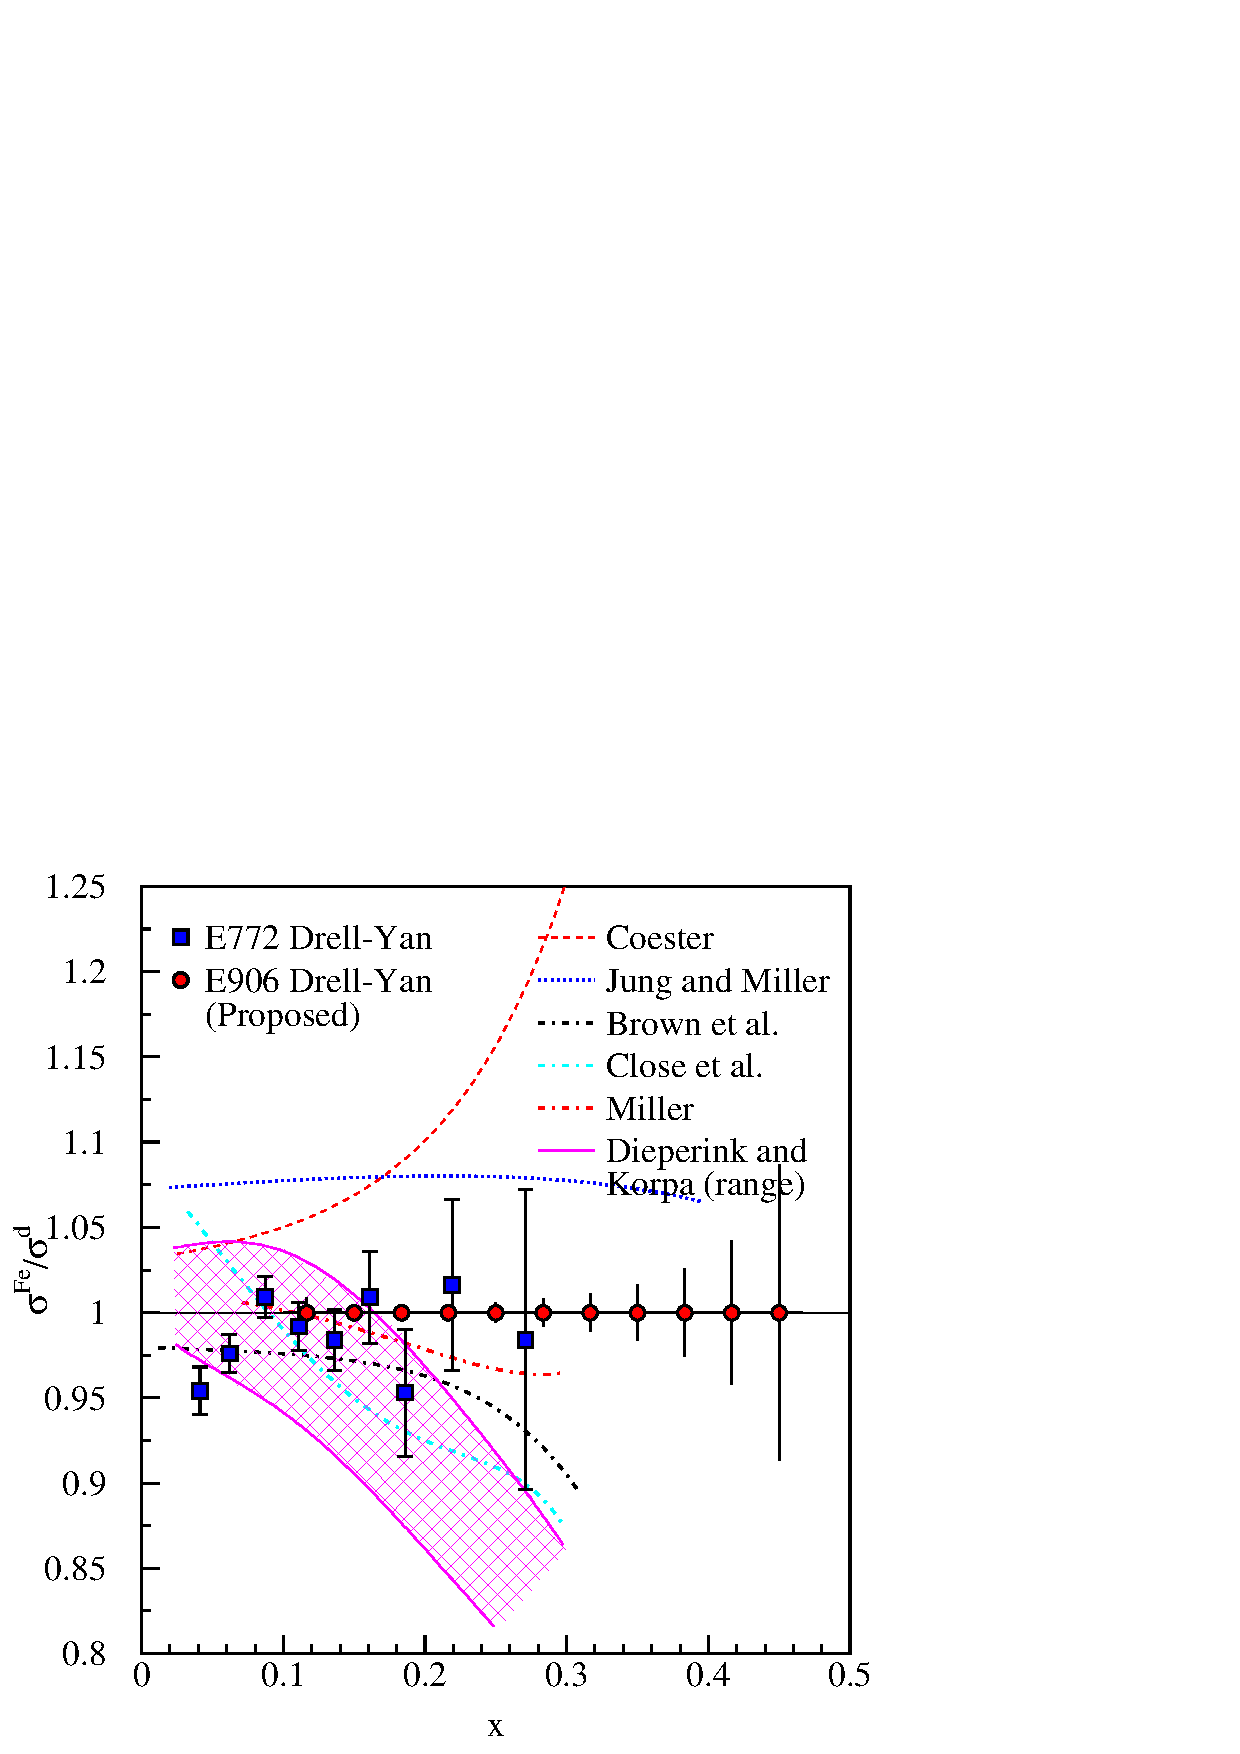
\includegraphics[width=0.4\textwidth]{nucpi_all_dfg.jpg}
\label{fig:projected} }
}
\caption{E772 and projected SeaQuest EMC Effect studies.}
\label{fig:e772_e906}
\end{figure}

The measurement to be made at SeaQuest is very simple by nature of the measurement.

\begin{equation}
R_A/d \equiv \frac{2}{A} \frac{d\sigma^{pA}/dx_1x_2}{d\sigma^{pd}/dx_1x_2}
\end{equation}

After adjusting for luminosity and beam time between targets, the crux of the analysis will actually be very simple.  The ratio of these per-nucleon cross sections will simply be the per-nucleon ratio of the yields of Drell-Yan dimuons between the $Fe$ and $D$ targets. By the nature of measuring ratios, many of the undesirable details such as acceptance or high-order QCD corrections simply \emph{go away}.  There are likely to be some corrections to the nuclear cross section due to isoscalar corrections \cite{Seely:2009gt, Cloet:2009qs} and quark energy loss in nuclear Drell-Yan \cite{duan-2007-50}, but the basic measurement will simply be the per nucleon ratio of the Drell-Yan yields.

Due to the rarity of the Drell-Yan process, along with the even rarer high-$x_2$ Drell-Yan, there is little-to-no information regarding the nuclear-to-deuterium cross sections. The only experiment to collect a fair amount of statistics has been Fermilab E772 (Figure \ref{fig:e772}), and that experiment was only able to explore up to $x_2=0.2$ before touching the EMC region. 

SeaQuest is poised to extend the range of E772 all the way out to $x_2=0.45$ (Figure \ref{fig:projected}), which is a considerably high value given the rarity of a beam quark experiencing a target anti-quark at that momentum. This range extension, along with higher precision in the $0.1<x_2<0.2$ would normally be good enough for any experiment, but the real excitement is that we're not sure what we'll see with Drell-Yan in the EMC region.

This recent hint at a link, first proposed by Higinbotham \cite{Higinbotham:2010ye}, connecting the EMC effect, short range correlations, and high-momentum nucleons has grown and developed to be the most promising theory in at least partially explaining a 28-year-old mystery. Perhaps the shape or slope of the EMC area will differ, indicating new phenomena, ushering in a new era of mysteries to uncover and theories to develop.

\section{The SeaQuest Spectrometer}
\subsection{FNAL Provisions, Temporary Setbacks}

The SeaQuest experiment will be carried out at the Fermi National Accelerator Laboratory in Batavia, IL.  Fermilab's facilities are capable of providing proton-antiproton collisions, meson beams, neutrino beams, and proton beams.  SeaQuest will me utilizing the latter for the purposes of our experiment.  Fermilab's accelerator chain will be providing a periodic burst of 120GeV protons from its main injector.  

The total number of protons promised to SeaQuest by Fermilab has been agreed on to be $7 \times 10^{18}$ protons over the lifetime of the experiment, which is expected to have a 2yr total run time.  Due to the way that beam is provided to all experiments, SeaQuest will be receiving $4\frac{s}{min}$ of beam at a rate of $2 \times 10^{12} \frac{protons}{s}$ during fully operational periods.  The luminosity  (number of particles per unit area per unit time times the opacity of the target) will be carefully controlled by adjusting the amount and distribution of the target materials.

There have been several setbacks that have affected the date of commissioning.  A leak was detected in the pipe that delivers beam to SeaQuest Hall, and a "sleeve" is currently being set inside the compromised beam pipe to re-establish a vacuum-tight avenue of beam delivery.  The delay in commissioning would have less severe implications if it weren't for the shut-down at Fermilab in the Spring of 2012 for the decommissioning of the Tevatron and the upgrading of the proton source.

There are currently efforts being undertaken to soften the blow that a shutdown would deal.  There have been discussions to double the amount of protons before the shutdown by delivering $8 \frac{s}{min}$ instead of 4.  Also, there is some consideration of pushing back the shut-down so that more significant statistics can be gathered by experiments that would not run after the shut-down.  This is significant to my personal research topic, as the study proposed here may depend solely on the data taken before the 2012 shut-down.

  \begin{figure*}
  \centerline{
    \mbox{\includegraphics[width=5.00in]{E906_Spectrometer.jpg}}
  }
  \caption{SeaQuest Spectrometer}
  \label{fig:spectrometer}
  \end{figure*}

\subsection{The SeaQuest Hall}
The SeaQuest spectrometer has a pleasantly simple hardware setup, as seen in Figure \ref{fig:spectrometer}.  There is a target table, a solid iron magnet that serves as a focusing magnet and a beam dump.  After this, there is an open-air spectrometer magnet and then a solid iron wall to further isolate all other particles but high-energy muons.  Along the way, there are four stations containing hodoscopes for triggering and drift chambers for particle tracking.  

The target table is able to hold five separate targets.  These targets will be able to move from target-target in between spills (a \emph{spill} being the four second bursts of beam).  This active movement of the targets will cancel out any long-term drifts incurred and will render the acceptance for nuclear and deuterium targets nearly the same, thereby minimizing systematic error.

Before the shut-down, the targets being used will be liquid $^1H$, liquid $^2H$, solid $Fe$, an empty flask, and a completely empty spot.  After the 2012 shut-down, the targets used will be liquid $^1H$, liquid $^2H$, solid $^{12}C$, $Ca$, and $W$, along with the empty flask and completely empty spot.  A pencil (long, thin) target will also be used to clearly identify the beam path.

The hodoscopes are arranged at station to allow fast input for the trigger to identify a \emph{good} event.  At each station, there are two planes, each sensitive to x or y.  Each plane is split into two along $y=0$ or $x=0$, and the aluminum frames are adjustable with regard to the separation.  Should the trigger rates get too high from our high-intensity beam, causing data acquisition dead-time, we should be able to separate particular \emph{"hot"} planes so that they avoid the beam path.

A coincidence trigger will be required from hodoscopes from three of the four stations in the x or y plane. Various specific or general trigger "roads", based on Monte Carlo information, may be implemented, limiting the number of triggered events to those that are most likely to contain dimuon events.

Once an event is triggered, data is gathered from the drift chambers and proportional tubes in order to see which specific wires and tubes were hit by a charged particle.  In these chambers are alternating grounded wires and anode wires kept at a high voltage.  When a charged particle passes through, it causes a localized cascade of ionization in the gas in the chamber, and this ionization is drawn to the wires, causing a current, or signal.  If one knows well the time it takes charges to drift through the gas (the space drift-time relation or SDTR), one can get a good idea of how from from the wire the signal passed through by carefully measuring the time of the pulse. 

The wire chambers are arranged so that there is a chamber with the wires oriented vertically along with a chamber behind it skewed from verticle (primed planes).  With the signals from a given wire chamber and its primed partner, one can arrive at a set of possible "stubs", or short, straight paths through which the particle could have traveled.  With proportional tubes, the amount of current deposited from the ionization is proportional to the energy of the particle, so additional information may be extracted.

\subsection{Particle Identification, Tracking, and Kinematic Reconstruction}
The only particles that we wish to detect in this experiment are muons; specifically dimuons, or two muons that share the same origin.  Muons, being leptons, only interact via the weak and coulombic interactions.  Also, since muons are 200 times as heavy as electrons, they are not as sharply accelerated by electromagnetic fields as electrons.  This means that they are able to penetrate dense material much more deeply than other hadronic material and electrons are able to.  The experiment is arranged with a solid iron focusing magnet and an iron wall in front of Station 4, both serving as absorbers, so that the only particles likely to make it through to all four stations are muons.

With this assumption, one can begin to track these muons since we know their mass ($105 MeV/c^2$).  For a given event, a set of aforementioned "stubs" are created at each set of drift chambers. The tracking then tries combining these stubs, using a lowest $\chi^2$ algorithm to find the best track to fit the set of stubs. This method is testable by taking Monte Carlo data, and then "digitizing" it, or turning space-points into detector elements, then reconstructing the tracks, and then comparing the result with the actual Monte Carlo tracks.

The bend angle through the magnet can be used to reconstruct the momentum of the muon.  One knows the behavior of a charged particle in a magnetic field obeys

\begin{equation}
	\frac{1}{r} = e \cdot \frac{B}{p}
\end{equation}
And it follows that
\begin{equation}
	\Delta\theta=\int\frac{ds}{r}=e\cdot \frac{\int B \cdot ds}{p}
\end{equation}
So, using the following units, we can approximate
\begin{equation}
	p[GeV/c] \simeq 0.2998 \frac{\int B[T] \cdot ds[m]}{\Delta \theta [rad]}
\end{equation}  	

When one knows the momenta of the two muons in a dimuon pair, you can add the two momenta together to get the four-momentum of the virtual photon, from which you have $\hat{s}$ or the invariant mass ($M_\gamma^2$) of the DY process.

Assuming that we know $\sqrt{s}$ for our beam configuration at the time, we can calculate the rest of our kinematic variables by Lorentz boosing the four-momentum from the lab frame into the $q\bar{q}$ center of mass frame, taking the longitudinal component, and calculating $x_F$ as
\begin{equation}
x_F = \frac{2 p_L}{\sqrt{s}}
\end{equation}
And then subsequently calculating $x_1$ and $x_2$ from the relations:
\begin{eqnarray}
x_F \approx x_1-x_2  \; \; \; \; \; \;  x_1 x_2 = \frac{M_\gamma^2}{s}
\end{eqnarray}

\section{Past, Present, and Future Work}
\subsection{Data Infrastructure}
My primary responsibilities in the SeaQuest collaboration have been in the form of designing, implementing, and maintaining the data infrastructure for our experiment.  When I first started with this research group, we decided to test out using a MySQL relational database to store our Geant Monte Carlo data, where the usual output has been to ROOT or PAW.  MySQL is an open-source relational database system that is well supported and widely used (Wikipedia, Amazon, Google, NASA, SLAC, etc.), and is well-known for its speed and versatility.

 \begin{figure*}
  \centerline{
    \mbox{\includegraphics[width=4.00in]{Softwarechain.jpg}}
  }
  \caption{SeaQuest software and data "chain".  The blue boxes are associated with the data acquisition (DAQ) systems. Yellow boxes are pieces of software written by our SeaQuest software group. Green boxes are aspects of the software chain implemented or stored via MySQL. The parts outlined in Red are those that are either partially or completely my responsibility.}
  \label{fig:softwarechain}
  \end{figure*}

There are several key operational benefits of this choice of infrastructure as well. The central nature of the data storage and access makes all of the up-to-date data universally available to collaborators at all times.  The mathematical capabilities of queries allows calculations and analysis to be performed on the data without trafficking it back and forth for analysis, thereby speeding up and simplifying the whole process. Other benefits include indexing, which can speed up regularly run queries, and the ability to treat simulation data exactly like run-time data for preparatory purposes.

The main effort in the infrastructure design has been to keep the data "naturally" organized, while keeping sizes manageable for queries as the experiment goes on. The data will be sorted out into blocks, corresponding to long (on the order of weeks) periods of run time. Each of these blocks, laid out in Figure \ref{fig:eer}, will be identical, and thereby easily queried and aggregated for final analysis.

 \begin{figure*}
  \centerline{
    \mbox{\includegraphics[width=4.00in]{EER.png}}
  }
  \caption{The atomic structure of our MySQL productions. A long period data taking is a run, which contains many 4s spills of beam, which corresponds to many CODA events, which corresponds to many hits and slow control values.  The calibration, mapping, and units tables help to make the hit and slow control information human-readable.}
  \label{fig:eer}
  \end{figure*}

\subsection{The deCODA}
The data acquisition (DAQ) is responsible for gathering data from valuable events and quickly storing the information into "flat" data files using a software system called CODA (CEBAF Online Data Acquisition).  These files are not human-readable, and can only be accessed from the local machines.  It has been my responsibility to develop and continue to augment and maintain a decoder, or "deCODA", which translates this raw information from CODA into the MySQL data structures that we have designed.

Each CODA file contains a set of "CODA events."  These events come in no particular order, and may contain any number of data formats, each of which change frequently to suit the needs of our data acquisition group. As a result, the deCODA has been designed in a very modular fashion in order to allow additional formats when added, or allow focused modification when a format is changed.

\subsection{Trigger Roads and Rates}

A trigger road is the set of hodoscope paddles that a particle passes through as it passes through the SeaQuest spectrometer. The particular interest is three-fold: to identify which roads are more likely roads from Drell-Yan-induced dimuons, and to identify which roads have a high noise-to-dimuon ratio, and to investigate what measures can be taken to decrease the trigger rate.

The first task is easily handled by running a large set of Drell-Yan dimuon-only Monte Carlo simulated data and histogramming hodoscope paddle combinations. A proton gun generator, which will simulate the "noise" for the experiment, would be used to perform the noise-to-dimuon ratio test; this is contingent, however, on the normalization of our dimuon generator and proton gun generator, which have not been in complete agreement with each other to date. 

The task of decreasing trigger rate is an important one. If, during data taking, our trigger rate is too high, we will effectively be losing data due to electronic dead time. The typical action in this case is to turn off certain trigger roads that have a high noise-to-dimuon ratio, as long as the loss of dimuons is not substantial. In our experiment, we have some degrees of freedom with our detector configuration. We can not only slightly move our Station 1 detectors, but we can also separate hodoscope planes at their center since each plane is composed of two rows of hodoscopes. 

The most natural place to implement this is in our Station 1 hodoscopes, which will be the ones fired off most rapidly by noise from the beam dump. After Station 1, most of the noise will be swept out of acceptance range by the open air magnet. Studies are currently under way to, via Monte Carlo data and MySQL query analysis, separate and/or move the Station 1 hodoscopes to effectively cut the trigger rate substantially without critically decreasing the trigger rate for good dimuon events.

\section{Conclusions}
Enhancement of quark distribution in nuclear medium can be measured at SeaQuest via the Drell-Yan hadron-hadron interaction. Such measurements of the ratio of cross sections of nuclear material to that of deuterium could contribute greatly to the understanding of the long-standing EMC Effect mystery. Additionally, an analysis of this ratio could provide independent evidence towards a newly emerged theory linking the EMC Effect to modifications in high-momentum nucleons \cite{PhysRevC.76.055206}, which in turn are dominated by NN SRC's and local nuclear density \cite{Weinstein:2010rt}. This is all-the-more highlighted by the fact that we will be the only Drell-Yan experiment currently investigating this phenomenon, and will be the first to explore it to such high $x_2$.

In the grand scheme of things, the data we take and the results we get will also help to better define the parton distribution functions. This goal is always of great importance, as the precise nuclear parton distribution functions are important components in finding new physics phenomena and determining such things as the electro-weak parameters, neutrino masses, and mixing angles in neutrino physics.

\bigskip
\bibliography{Dannowitz_Preliminary_Paper}
\bibliographystyle{plain}

\end{document}